\section{Empirical Results}
\label{sec:empirical-results}
To evaluate the algorithms presented in Section~\ref{sec:flexible-resource-allocation-mechanisms},
this sections analysis the different algorithms, the possibility of misreporting task attributes,
the effect of the server resource capacity and online task arrival.

To do evaluate our algorithms, synthetic models have been used to generate servers and tasks where
each attribute was taken from a Gaussian distribution. The reason this was done was due to there not
being a de facto standard to test cloud computing resource allocation algorithms and that those used
in related work do not consider a deadline for a task.

\subsection{Evaluation of the Greedy Algorithm}
\label{subsec:evaluation-of-the-greedy-algorithm}
To compare the greedy algorithm to the optimal elastic allocation, a branch and bound was implemented to solve the
optimisation problem in section~\ref{subsec:optimisation-problem}. In order to compare to fixed speed equivalent models,
the minimum total resource required to run the job is found and set as the resource speeds for all of the tasks, with
the optimal solution for running the job with the fixed speeds is found as well. To implement the greedy mechanism, the
value density function was $\frac{v_j}{s_j + w_j + r_j}$, server selection was
$\text{argmin}_{\forall i \in I} S^{'}_i + W^{'}_i + R^{'}_i$ and the resource allocation was
$\min s^{'}_j + w^{'}_j + r^{'}_j$ for job $j$ and servers $I$.

\begin{figure}[h]
    \centering
    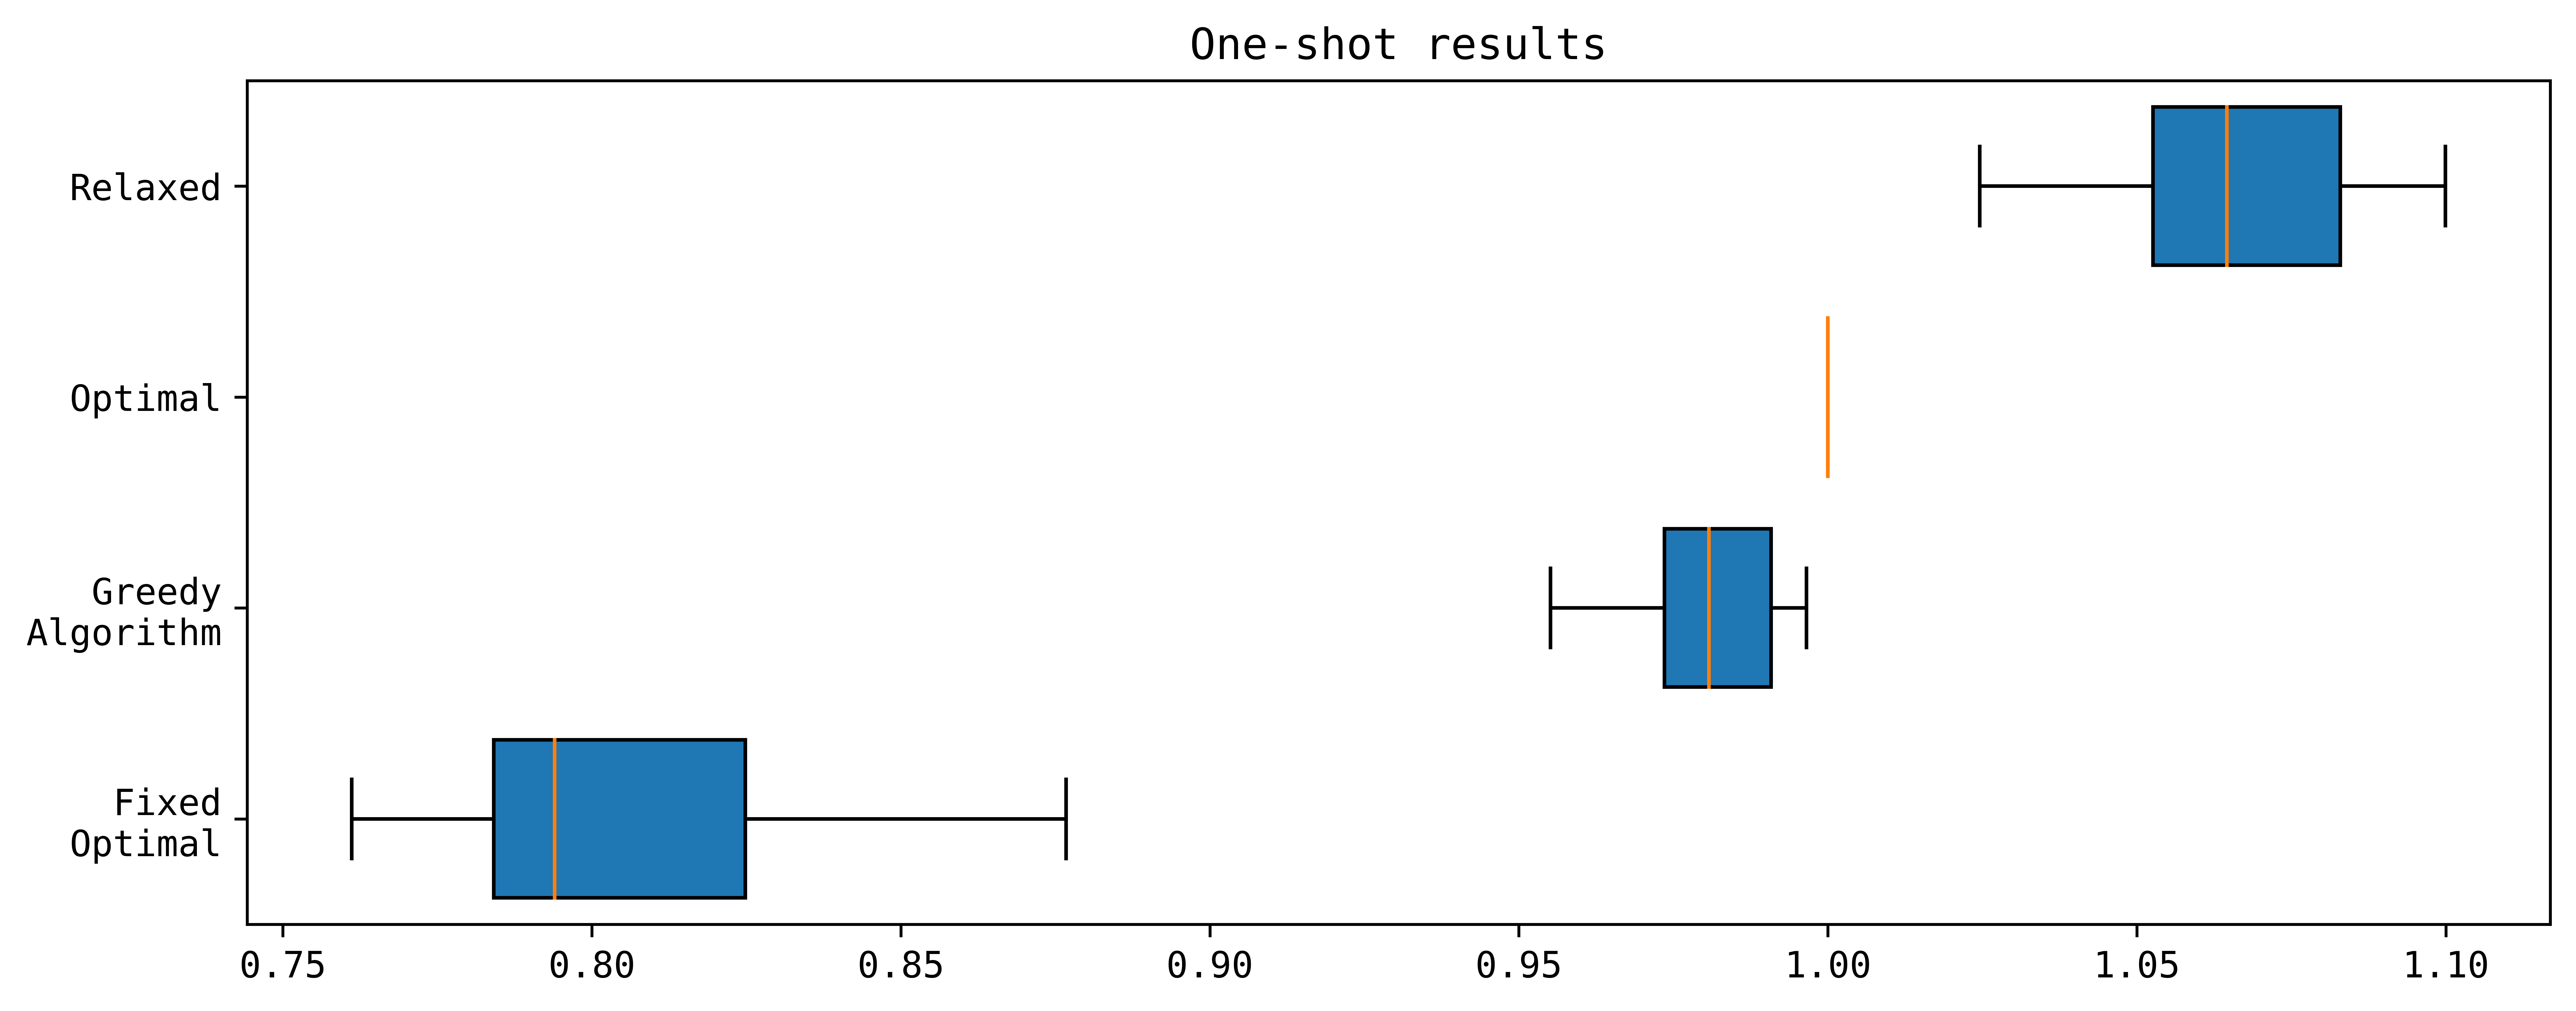
\includegraphics[width=\linewidth]{figs/greedy/greedy_algorithms.png}
    \caption{Comparison of the social welfare for the greedy mechanism, optimal, relaxed problem, time limited branch and bound}
    \label{fig:greedy-mechanism-comparison}
\end{figure}
As figure~\ref{fig:greedy-mechanism-comparison} shows, the greedy mechanism achieves 98\% of the optimal solution for
the small models, the mechanism achieves within 95\% for larger models. In comparison, the fixed allocation achieves
80\% of the optimal solution and always does worse than the social welfare of the greedy mechanism.

\subsection{Evaluation of the Auction mechanisms}\label{subsec:evaluation-of-the-auction-mechanisms}
Figure~\ref{fig:auction-mechanisms-comparison} compares the social welfare of the auction mechanisms: VCG auction,
fixed resource speed VCG auction, critical value auction and the decentralised iterative auction with different price
change variables.

\begin{figure}[h]
    \centering
    \includegraphics[width=\linewidth]{figs/auctions/auctions_results.png}
    \caption{Comparison of the social welfare for the auction mechanisms}
    \label{fig:auction-mechanisms-comparison}
\end{figure}

\subsection{Effectiveness of Decentralised Iterative Auction Heuristics}
\label{subsec:effectiveness-of-decentralised-iterative-auction-heuristics}
\begin{figure}[h]
    \centering
    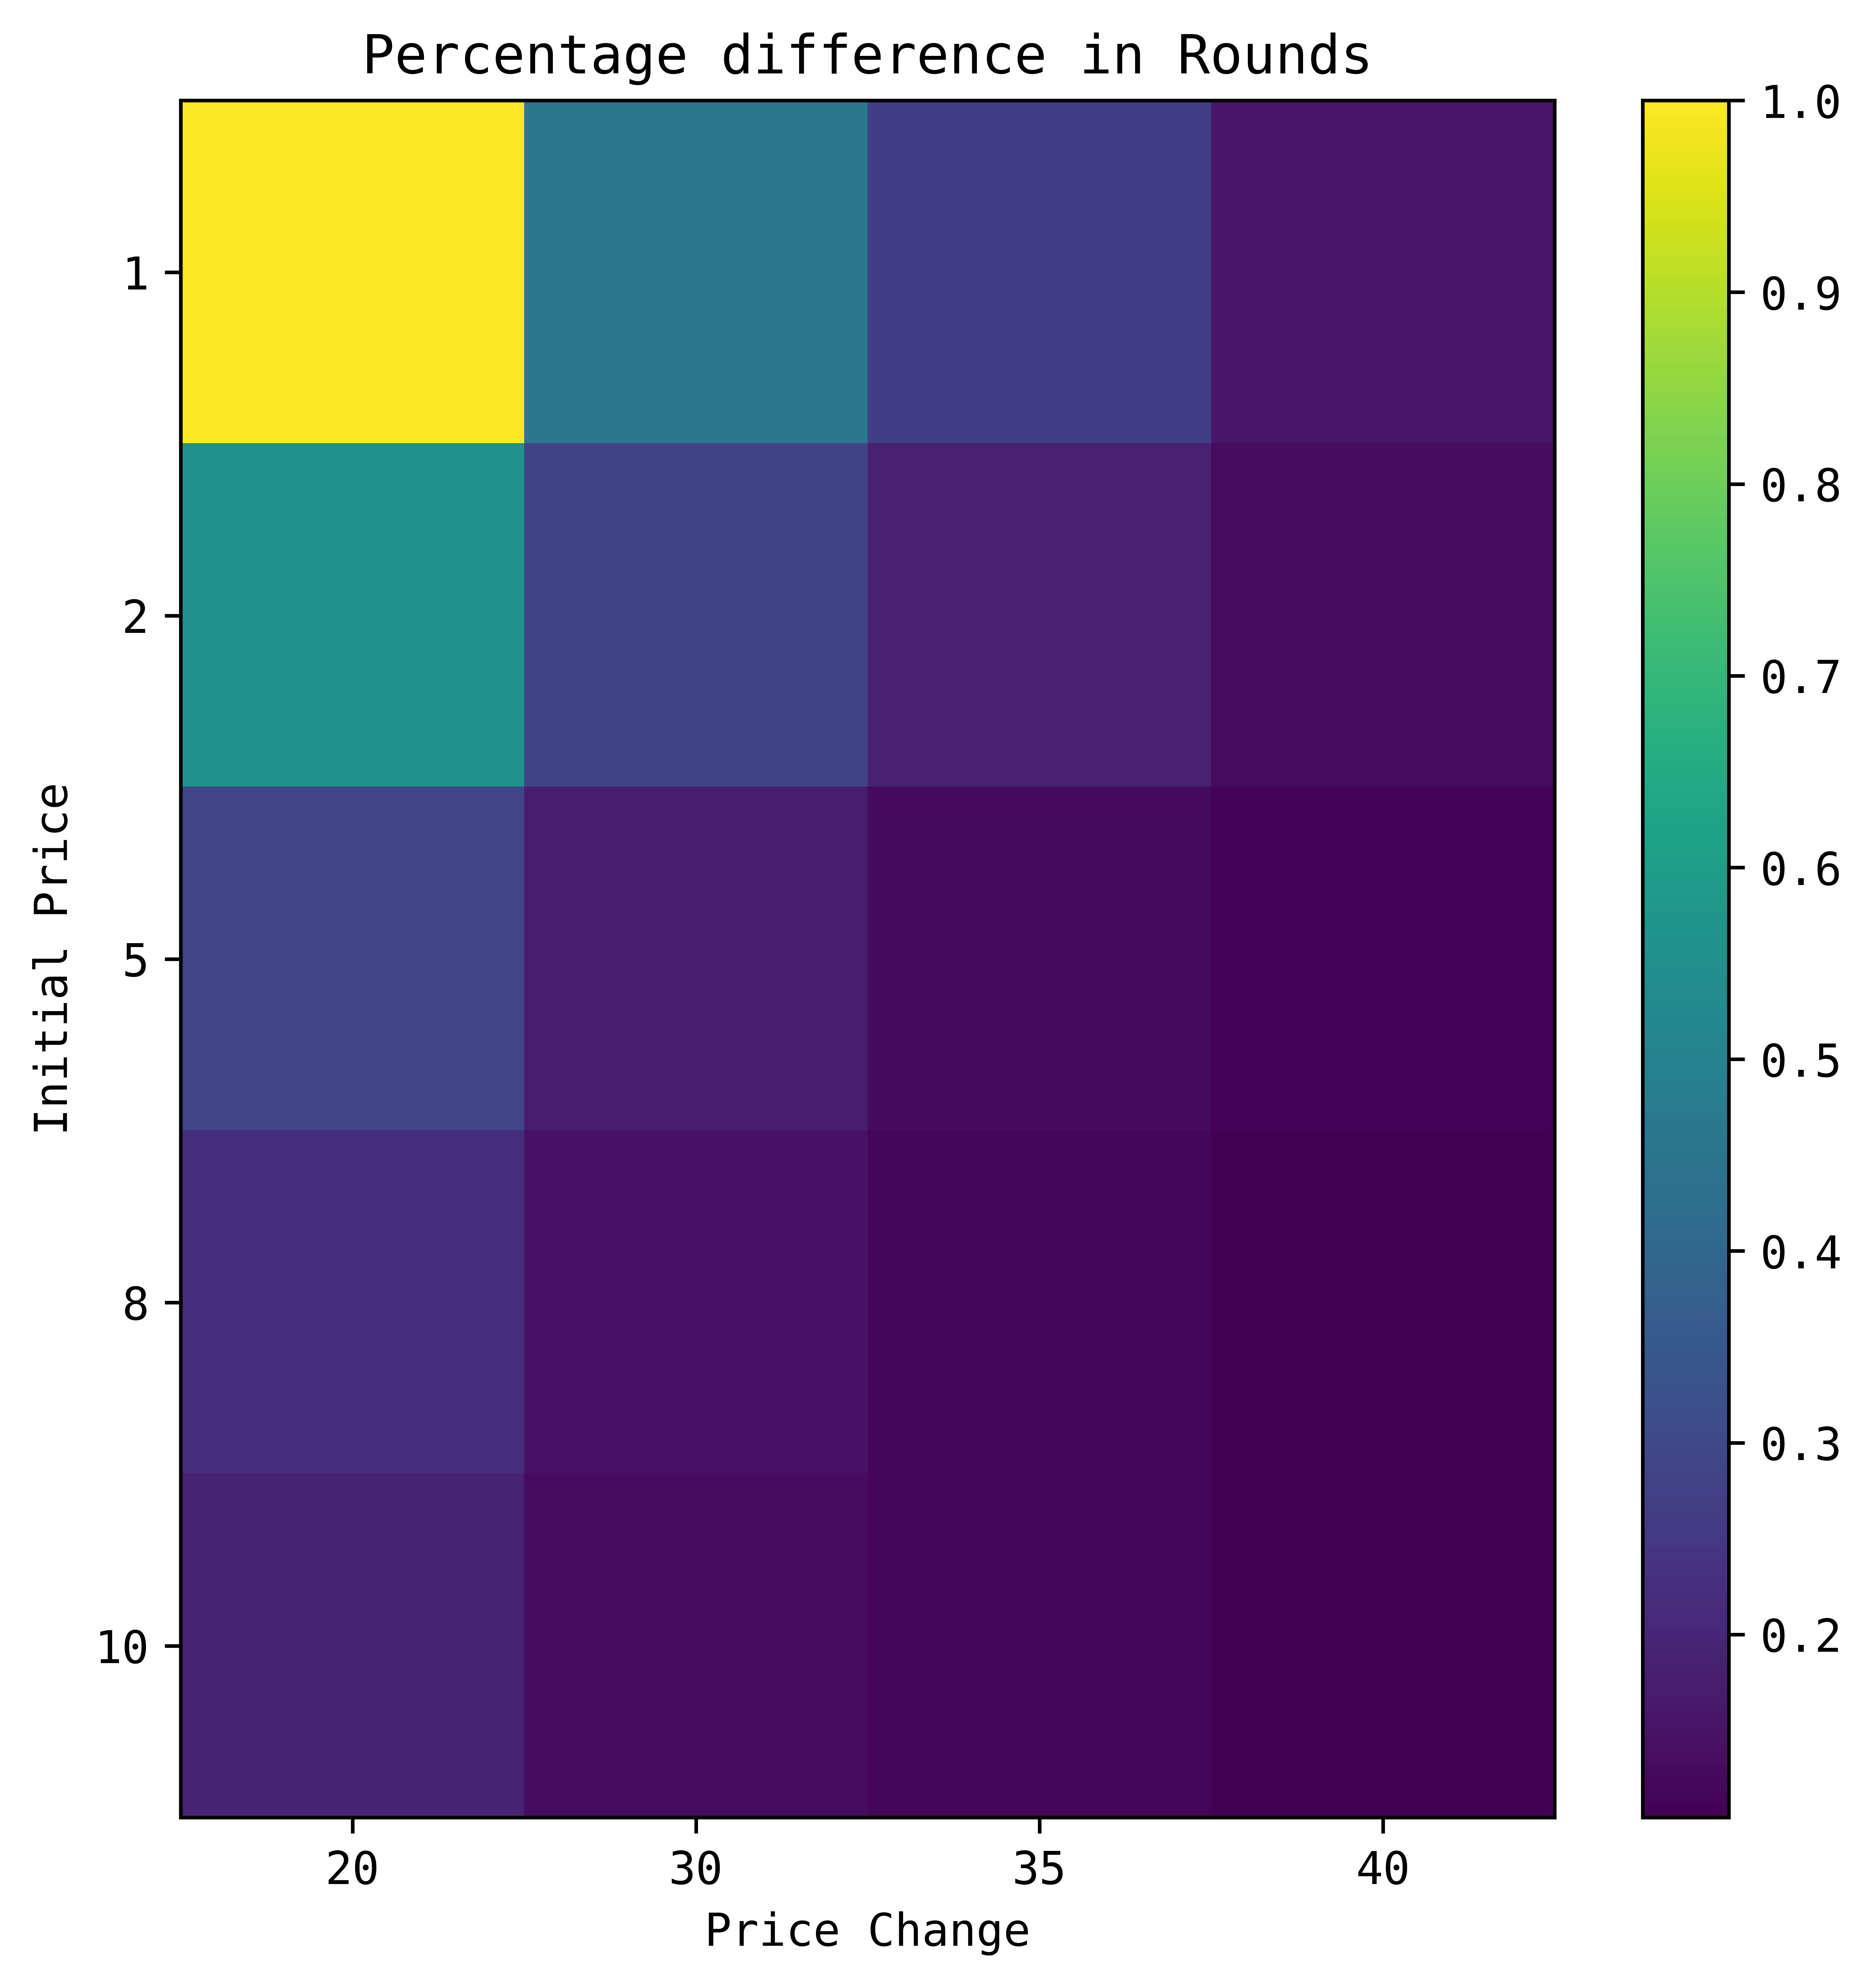
\includegraphics[width=0.45\linewidth]{figs/dia_heuristics/rounds_grid.png}
    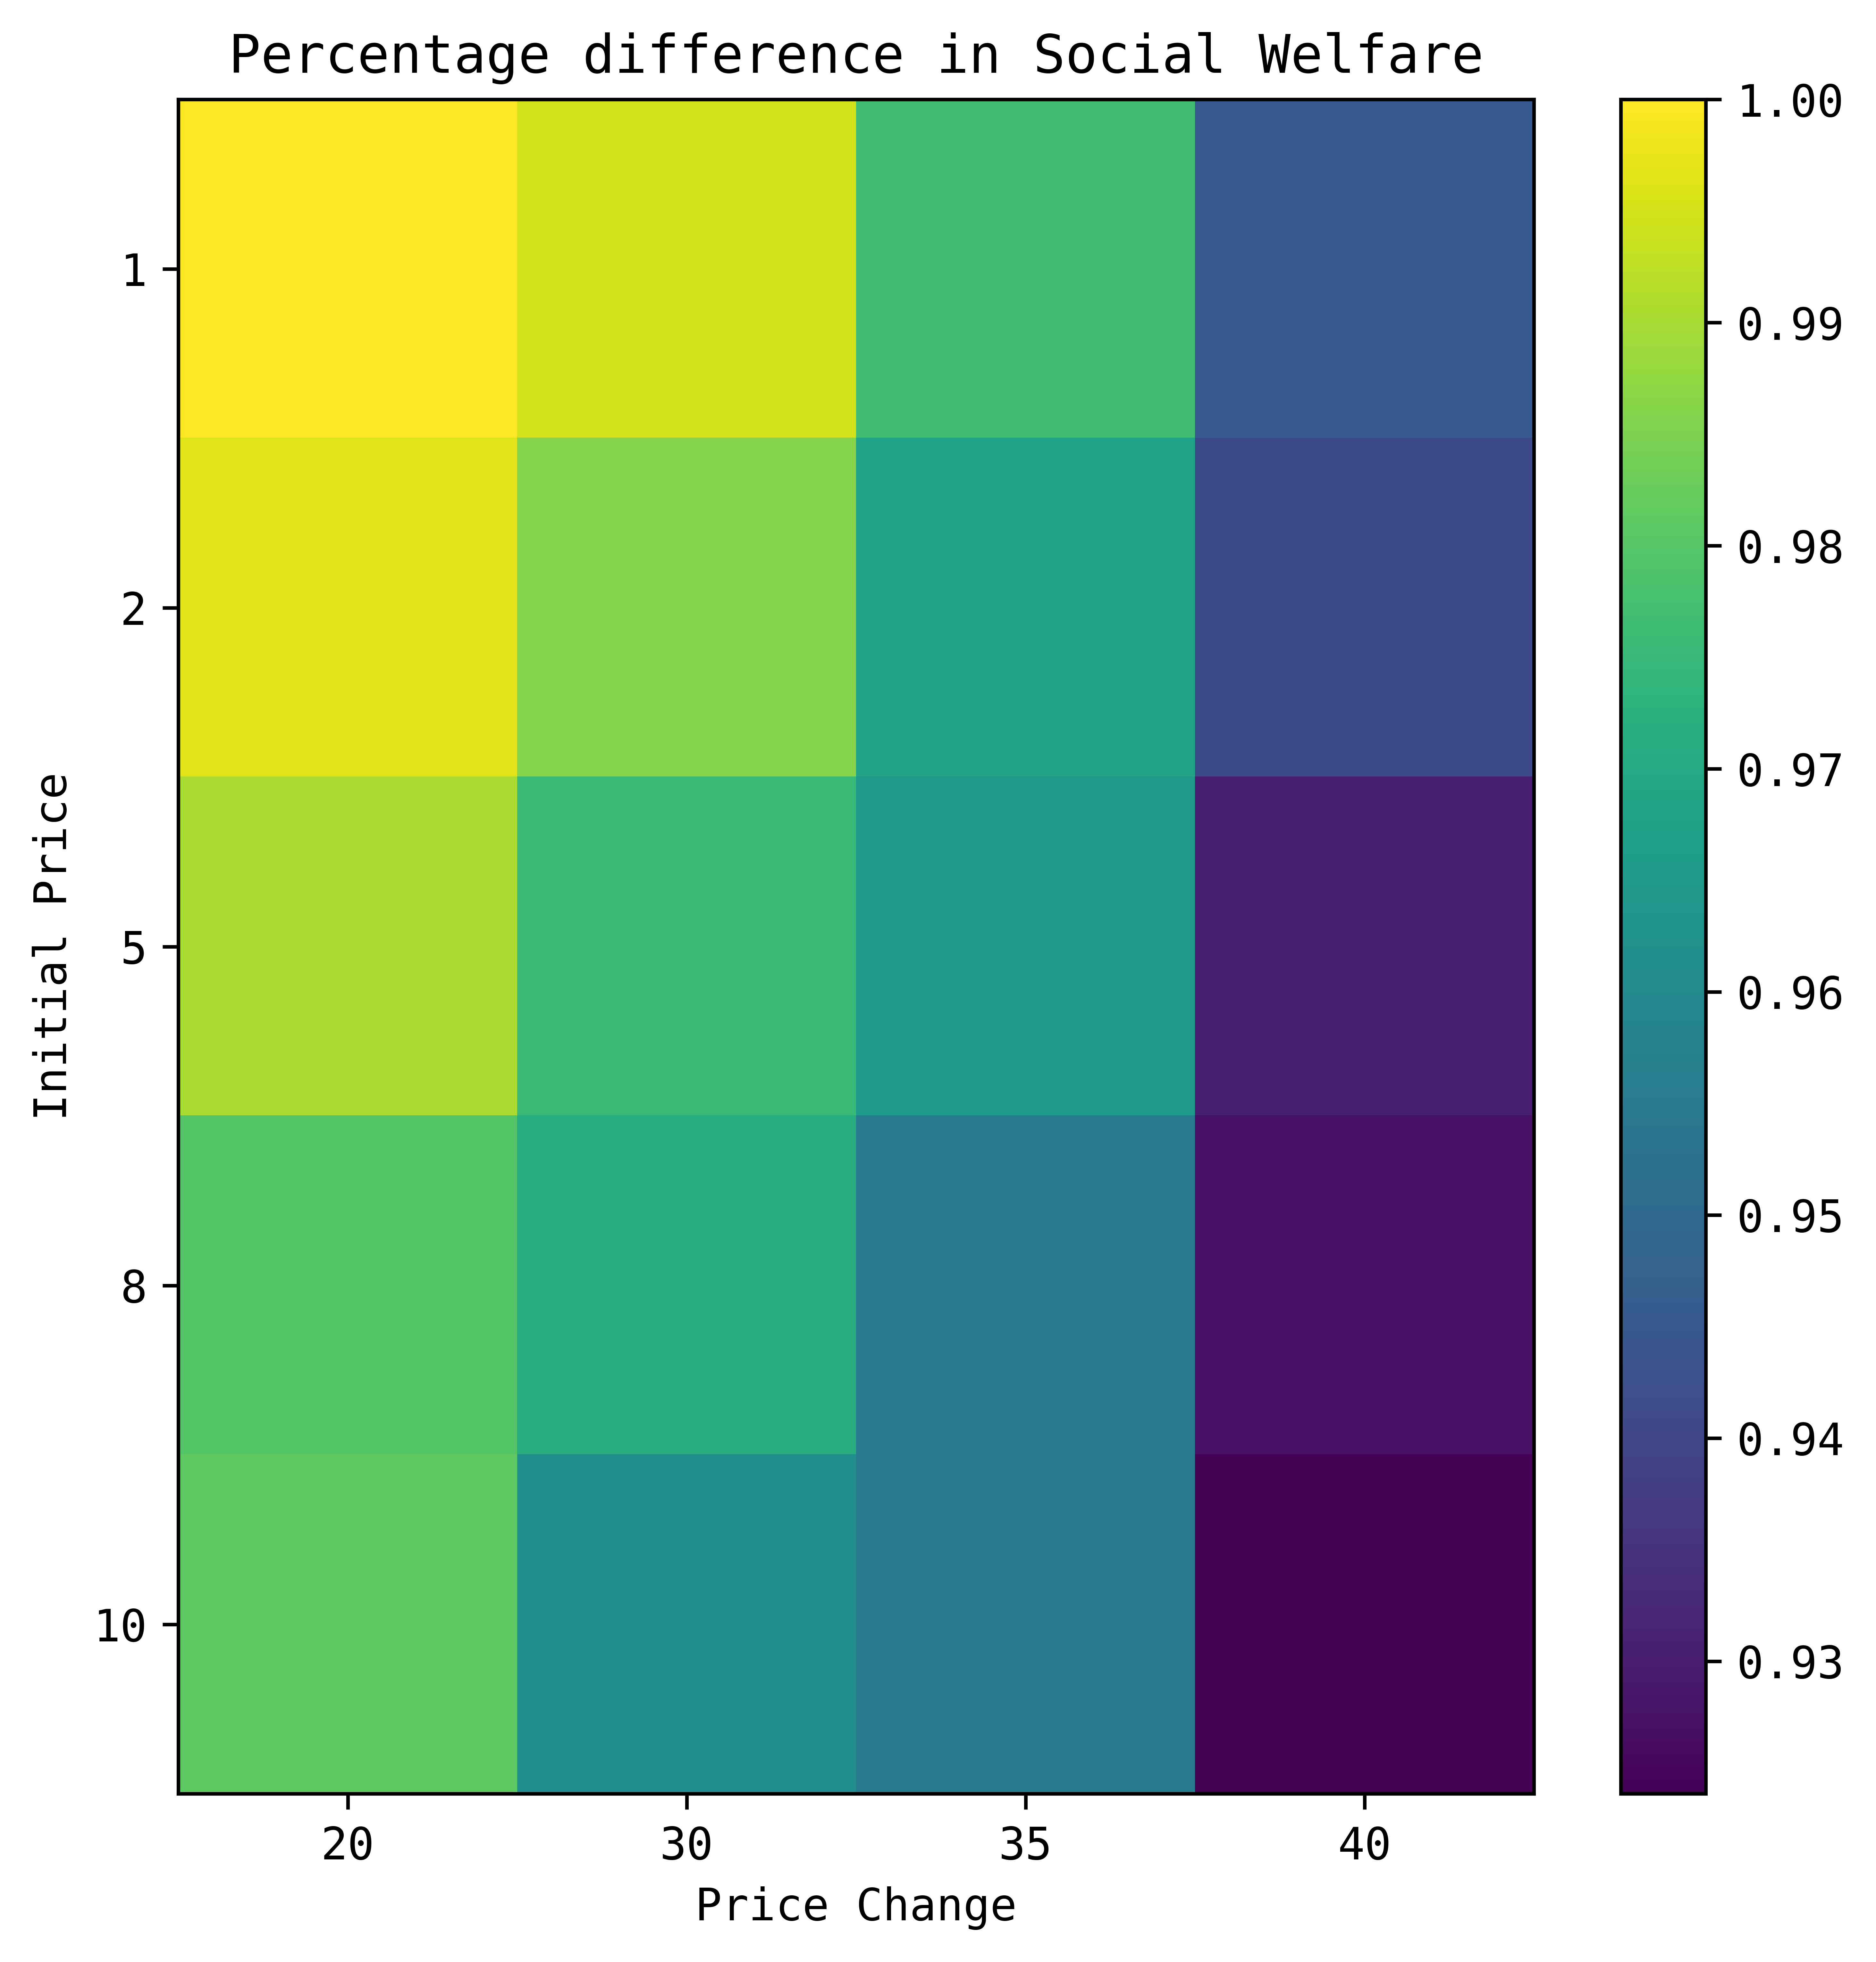
\includegraphics[width=0.45\linewidth]{figs/dia_heuristics/social_welfare_grid.png}
    \caption{Grid search of difference server price change and task initial cost}
    \label{fig:dia_sw_rev_grid_search}
\end{figure}

\begin{wrapfigure}{r}{0.45\linewidth}
    \centering
    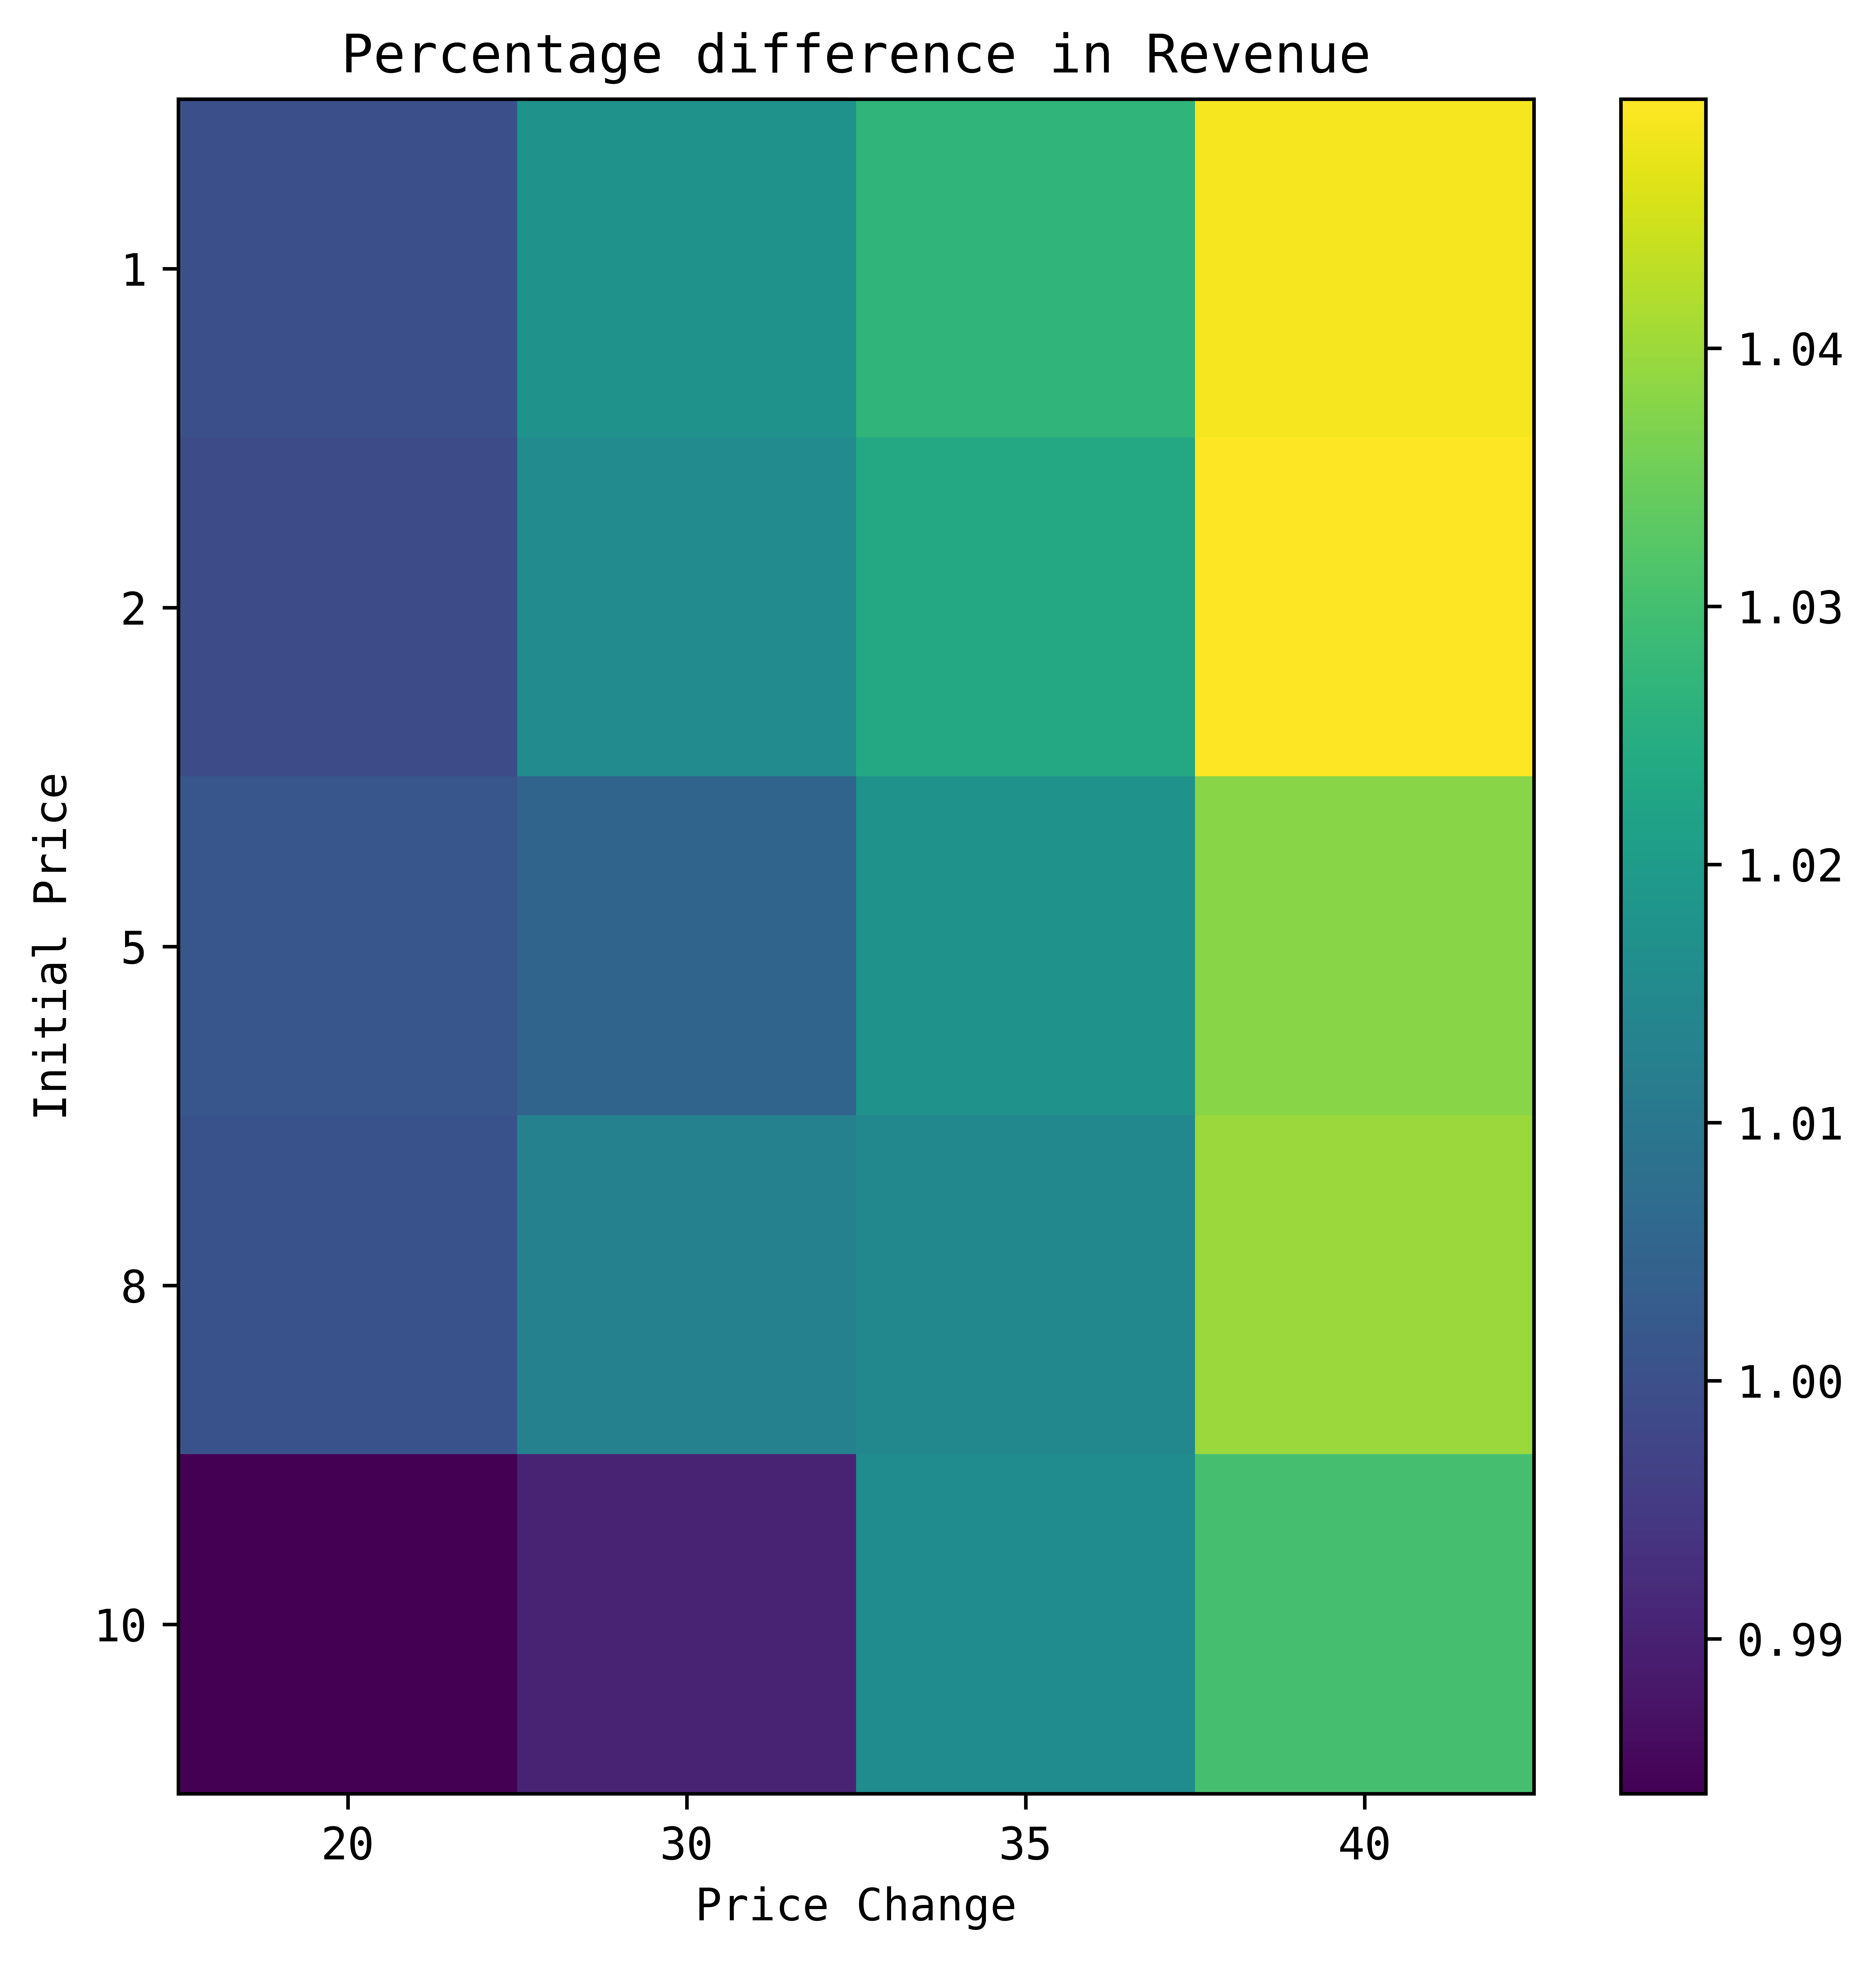
\includegraphics[width=\linewidth]{figs/dia_heuristics/revenue_grid.png}
    \caption{Grid search for rounds}
    \label{fig:dia_rounds_grid_search}
\end{wrapfigure}

Within the context of edge cloud computing, the number of rounds for the decentralised iterative auction is important
to making it a feasible auction as it is proportional to the time required to run. We investigated the effect of two
heuristic on the number of rounds and social welfare of the auction; the price change variable and initial cost
heuristic. With an auction using as minimum heuristic values for the price change and initial cost,
figure~\ref{fig:dia_rounds_grid_search}, on average 400 rounds were required for the price to converge while an auction
using a price change of 10 and initial cost of 20 means that only on average 80 rounds are required, 5x less. But by
using high initial cost and price change heuristics, this can prevent tasks from being allocated,
figure~\ref{fig:dia_sw_rev_grid_search}, shows that the difference in social welfare is only 2\% from minimum to
maximum heuristics.

\subsection{Possibility of Task Mutation in Decentralised Iterative Auction}
\label{subsec:possibility-of-task-mutation-in-decentralised-iterative-auction}
%Mutation auction
%\begin{figure}
%    \centering
%    \includegraphics[width=\linewidth]{figs/mutation/}  %% TODO update with the mutated png
%    \caption{Difference in task price to a truthful task and misreported task}
%    \label{fig:auction-mutation}
%\end{figure}
%As the decentralised iterative auction presented in section~\ref{subsec:decentralised-iterative-auction} is not
%incentive compatible, it is possible that misreporting of task attribute can decrease the price paid by a task.
%Figure~\ref{fig:auction-mutation} is a scatter graph of the a task (in orange) and the price of a misreported task
%(in blue). Misreported task were generated by increase the task resource requirements or by decreasing the task value
%or deadline that would substituted for the original truthful task. As the figure clearly shows, in almost all cases of
%mutation causes the

\subsection{Effect of Server Resource Capacity Ratio}
\label{subsec:affect-of-server-resource-capacity-ratio}
Due to the elasticity in the resources, an advantage of such a system is the ability for server to more efficiently
distribute their resources particularly when certain server resources are scarce. To confirm this, a models were
generated where for a range of ratios, a server's bandwidth and computation resources are redistributed to fit the
ratio. At such a point, the greedy algorithm using the settings from
subsection~\ref{subsec:evaluation-of-the-greedy-algorithm} were used, the optimal flexible solution and the optimal
fixed solution.

\begin{figure}[h]
    \centering
    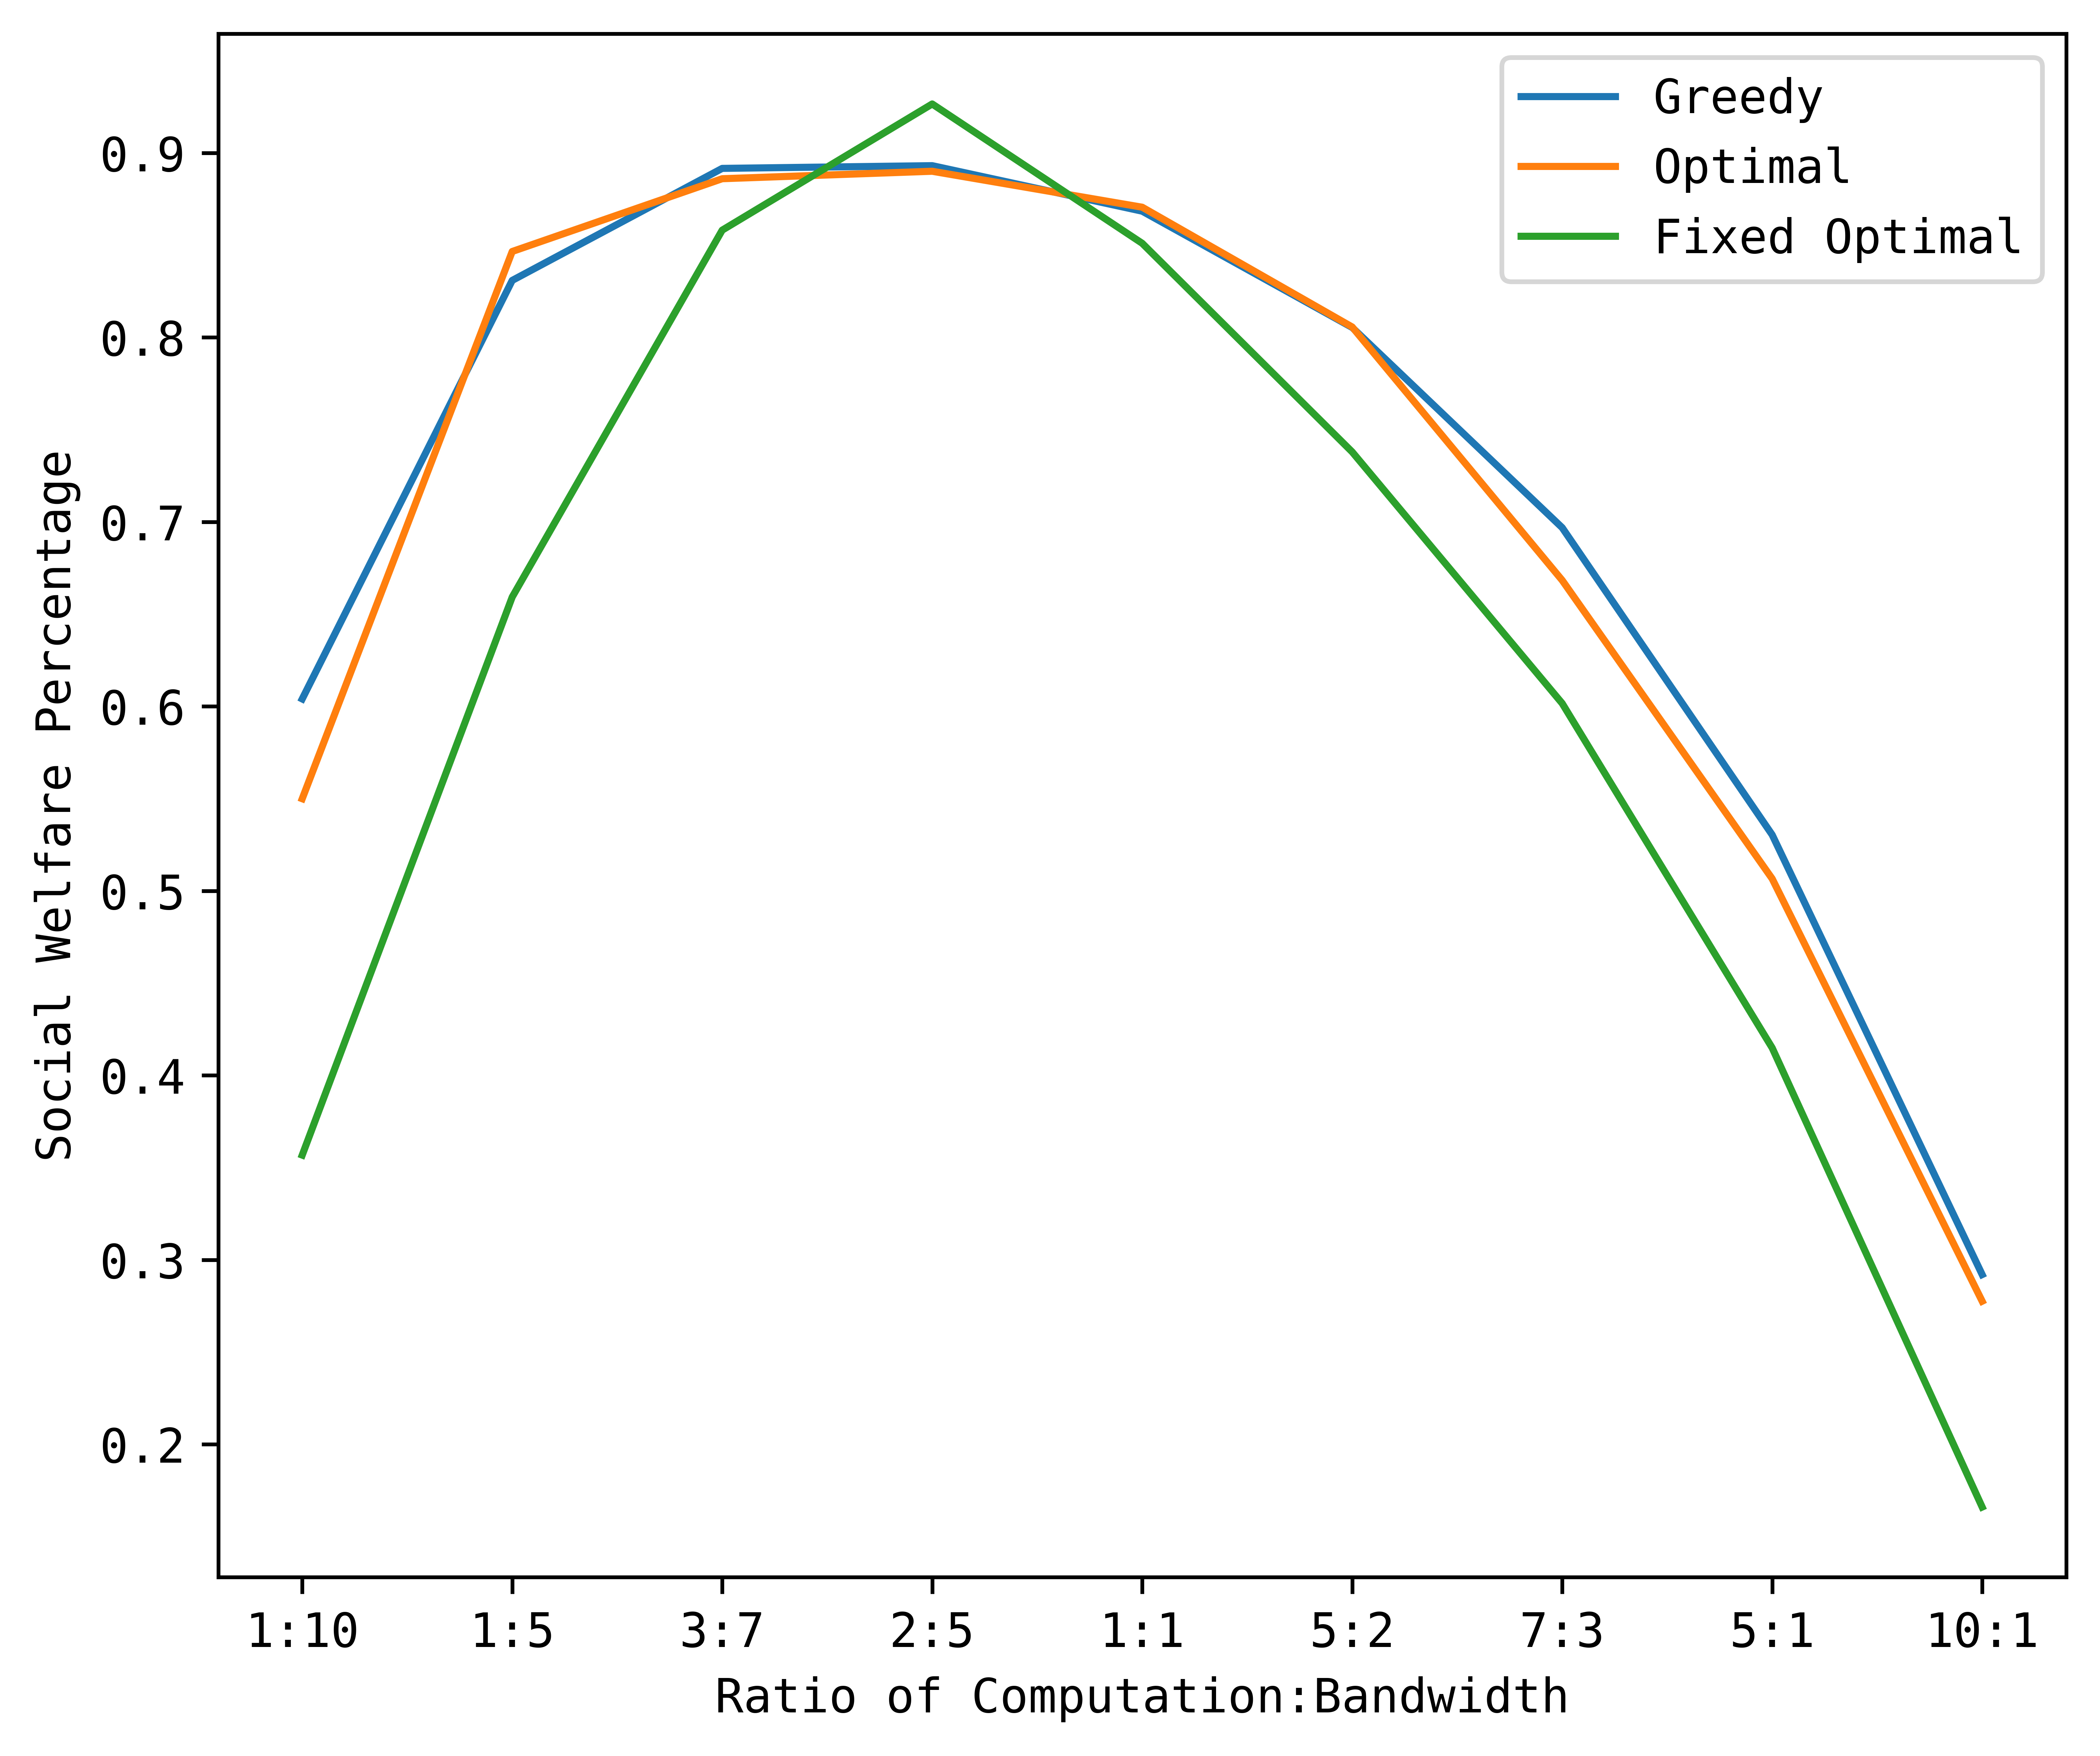
\includegraphics[width=0.45\linewidth]{figs/resource_ratio/social_welfare_percentage.png}
    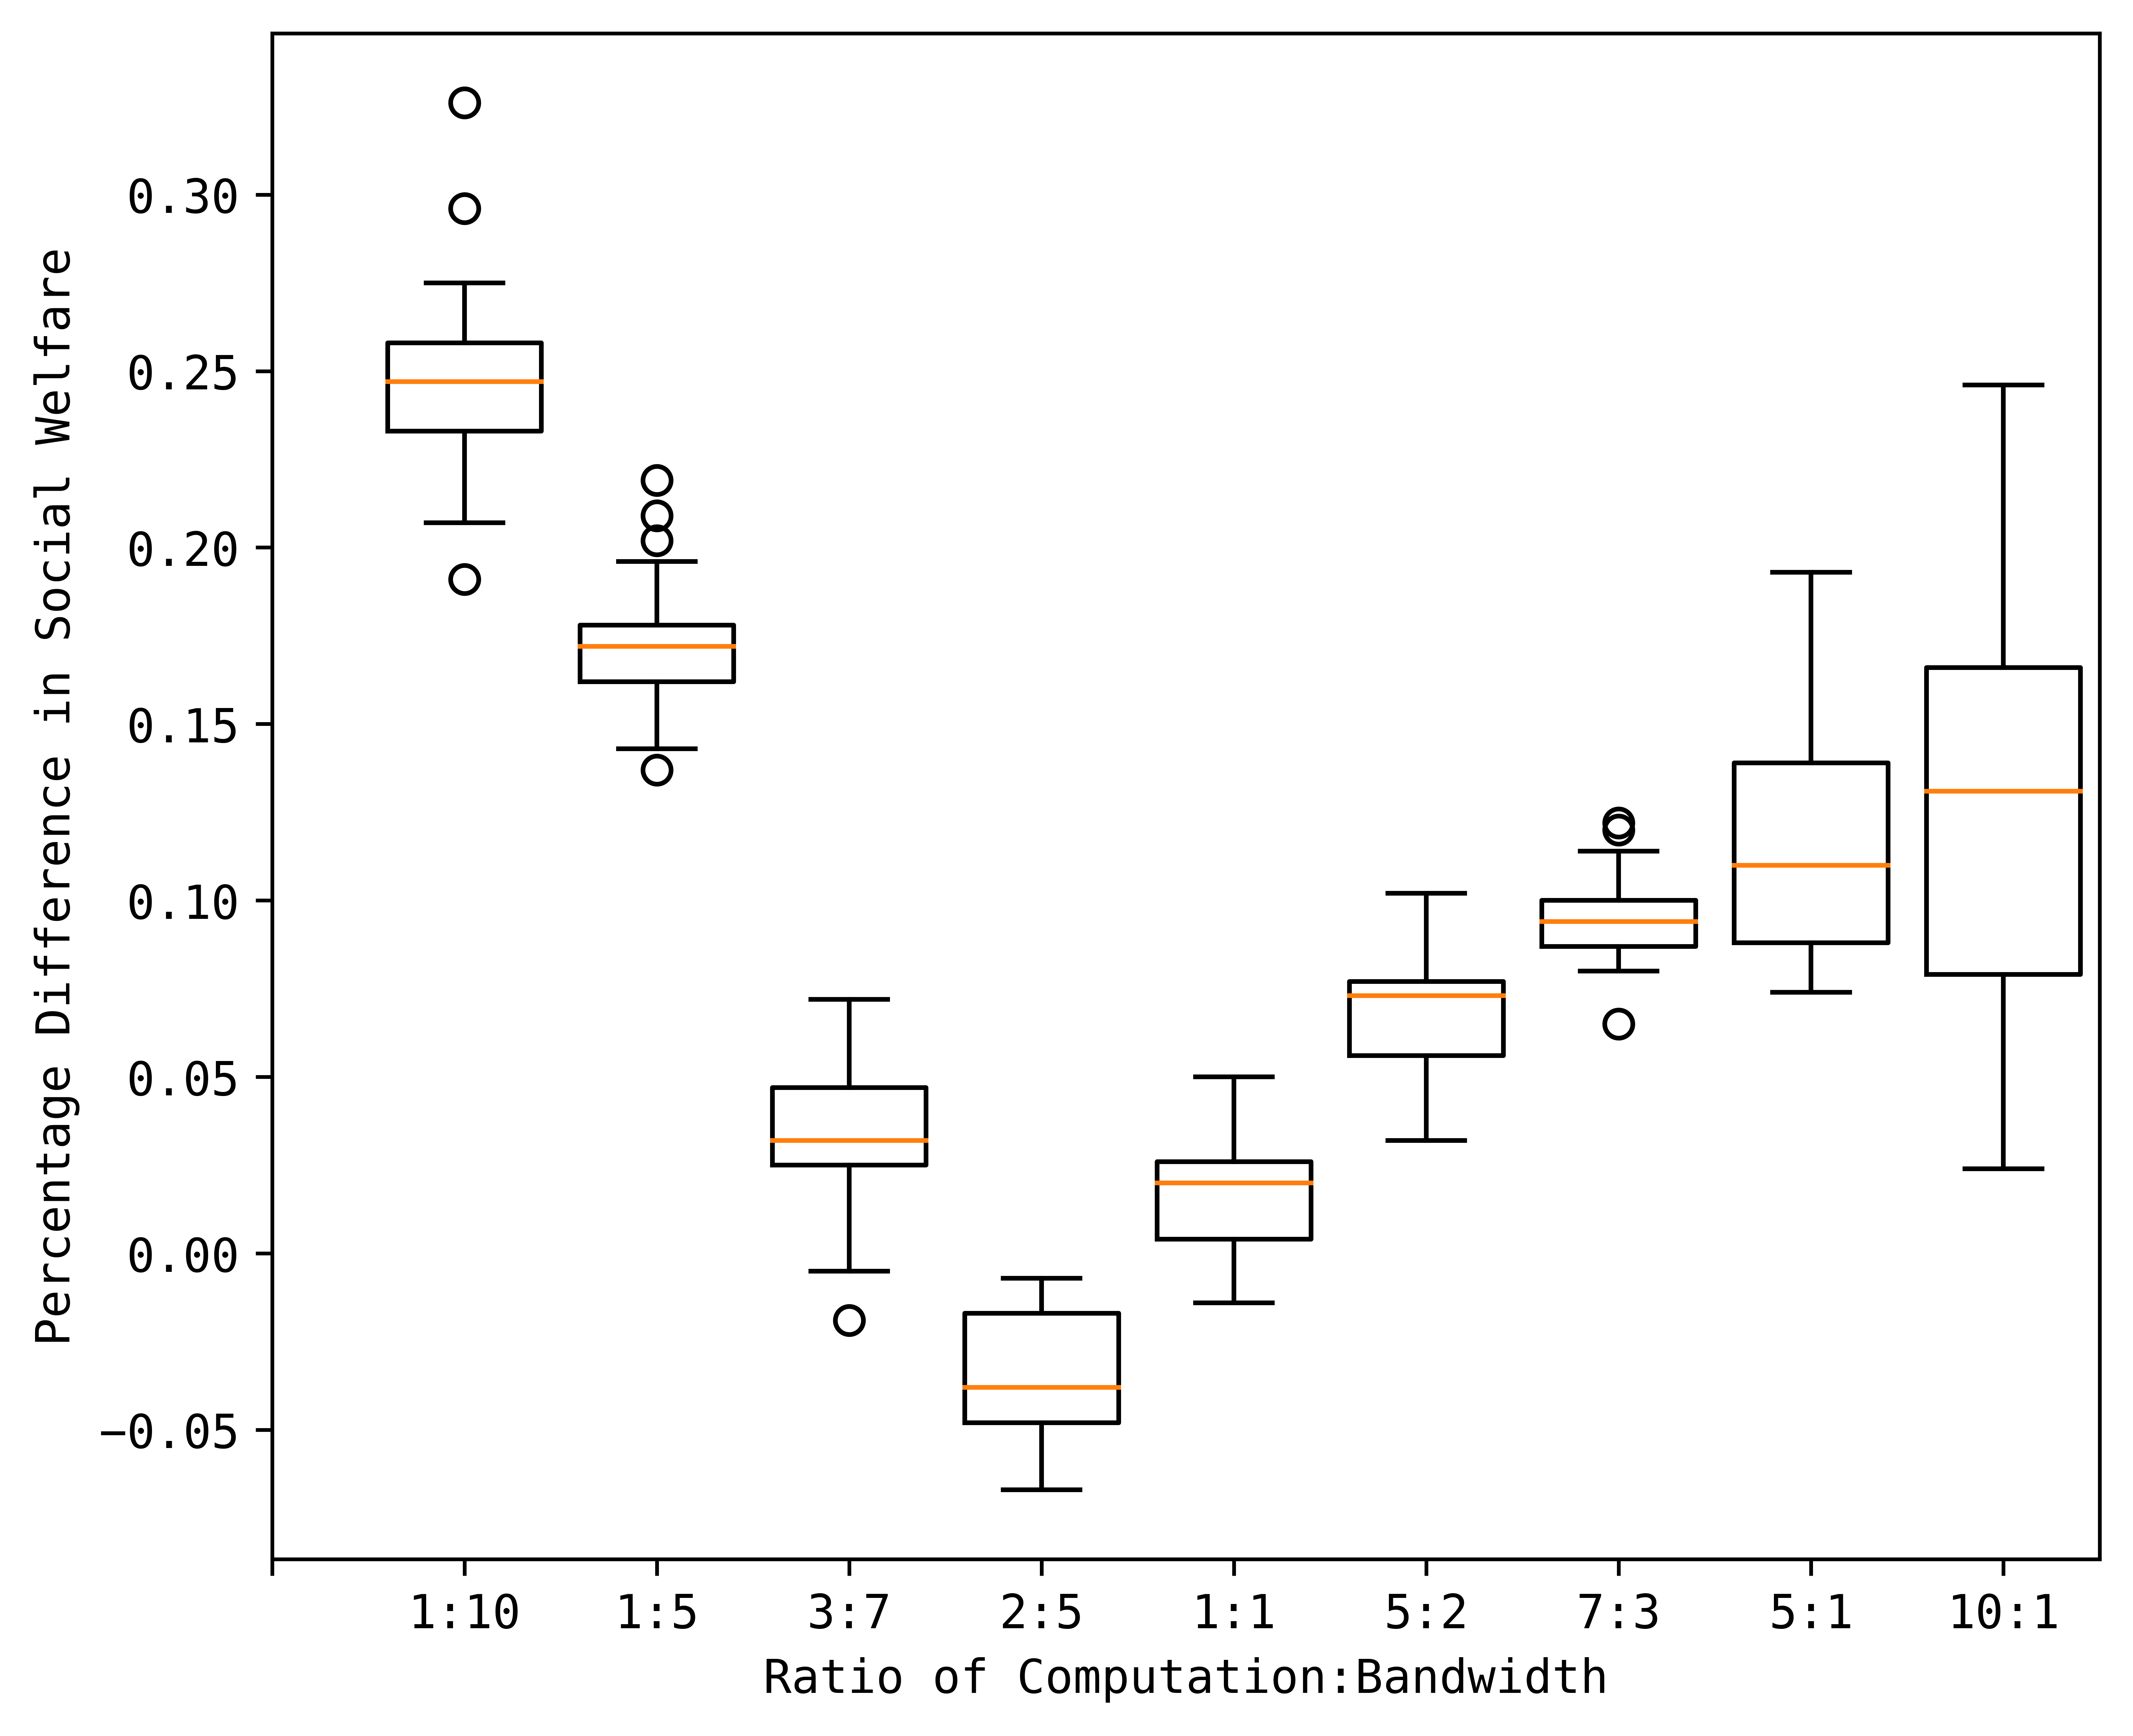
\includegraphics[width=0.45\linewidth]{figs/resource_ratio/social_welfare_difference.png}
    \caption{Social welfare}
    \label{fig:resource-ratio-social-welfare}
\end{figure}

This can be seen more clear by plotting the average server resource usage each of the ratios.
\begin{figure}[h]
    \centering
    \includegraphics[width=\linewidth]{figs/resource_ratio/server_resource_usage.png}
    \caption{Server resource usage}
    \label{fig:resource-ratio-server-resource-usage}
\end{figure}

\subsection{Batching verse Online task allocation}
\label{subsec:batching-verse-online-task-allocation}
* Explain the reason for the evaluation
* Add figure
* Explanation for DIA advantage as can run over the batch not just at the end

\begin{figure}[h]
    \centering
    \includegraphics[width=\linewidth]{figs/online/online_batch_lengths.png}
    \caption{Online batch lengths}
    \label{fig:batch-task-allocation}
\end{figure}